\documentclass[bigger, aspectratio=169]{beamer}

\usepackage{booktabs}
\usetheme{metropolis}
\metroset{block=fill}
\setbeamercolor{background canvas}{bg=white}
\usepackage[english]{babel}
\usepackage[utf8]{inputenc}
\usepackage{mathtools,amssymb,amsthm}
\usepackage{graphicx}

\title{Better Model, Worse Predictions}
\subtitle{The Dangers in Student Model Comparisons}

\author{Jaroslav \v{C}ech\'ak \and Radek Pel\'anek\\[5mm]
%Masaryk University Brno\\
%Czech Republic
%
\includegraphics[width=.35\linewidth]{figures/al-logo}\\[3mm]
}

\newcommand{\img}[2]{
  \begin{center}
    \includegraphics[width=#1\linewidth]{figures/#2}
  \end{center}
}

\newcommand{\mute}[1]{
  {\color{gray}{#1}}
}

\date{\vfill AIED 2021\hfill 
\includegraphics[width=.35\linewidth]{figures/al-logo}}

\begin{document}

\frame{\titlepage}


\begin{frame}
	\frametitle{Context}
	\begin{enumerate}
		\item Collect correctness of student responses to items.
		\item Define multiple mappings of items to concepts.
		\item Fit models' parameters to collected data.
		\item Compare models' performances and select the best one.
		\item Interpret fitted parameters. 
	\end{enumerate}
\end{frame}

\begin{frame}
	\frametitle{Additive Factor Model (AFM)}
	A logistic model for predicting answer correctness based on
	\begin{itemize}
		\item student's skill,
		\item difficulties of concepts involved in an item, and
		\item student's practice history.
	\end{itemize}  
	
	\begin{center}		
		\begin{equation*}
		P(Y_{ij}|\alpha, \beta, \gamma) = \sigma\left(z_{ij}\right)
		\end{equation*}
		\begin{gather*}
			z_{ij} = \biggl(
			\underbrace{%
				\vphantom{\sum_{k=1}^K \beta_k q_{jk}}  % to shift underbrace down
				\alpha_i
			}_{\substack{\text{student's}\\\text{prior skill}}} 
			+ \underbrace{\sum_{k=1}^K \beta_k q_{jk}}_{\substack{\text{concepts'}\\\text{easiness}}} 
			+ \underbrace{\sum_{k=1}^K \gamma_k q_{jk} t_{ik}}_{\substack{\text{student's}\\\text{learning}}}
			\biggr)
		\end{gather*}
		
	\end{center}
\end{frame}

\begin{frame}
	\frametitle{AFM}
	\begin{center}
		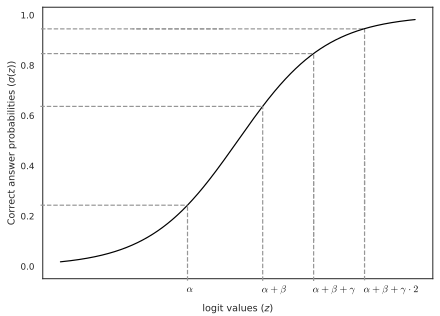
\includegraphics[width=0.7\linewidth]{figures/afm_explanation}
	\end{center}
\end{frame}

\begin{frame}
	\frametitle{Treatment of student parameters}
	\begin{itemize}
		\item Parameter fitting details rarely discussed.
		\item Student skill parameters ($\alpha$) are crucial for model evaluation.
		\item \textbf{Mismatch between assumed and actual student skill distribution causes problems.}
	\end{itemize}
\end{frame}


\begin{frame}
	\frametitle{Simulations}
	motivation
	\begin{itemize}
		\item known ground truth
		\item known data generation mechanism
		\item ability to isolate and exaggerate some aspect 
	\end{itemize}
		
	setting
	\begin{itemize}
		\item single concept
		\item $\alpha$ follows $\mathcal{N}(0, 1)$, $\mathcal{N}(0, 2^2)$, or $\mathcal{N}(0, 3^2)$
		\item AFM used as data generation method
	\end{itemize}
\end{frame}

\begin{frame}
	\frametitle{Results}
	AFMs with fitted parameters outperformed AFM with ground truth parameters
	
	\begin{center}
		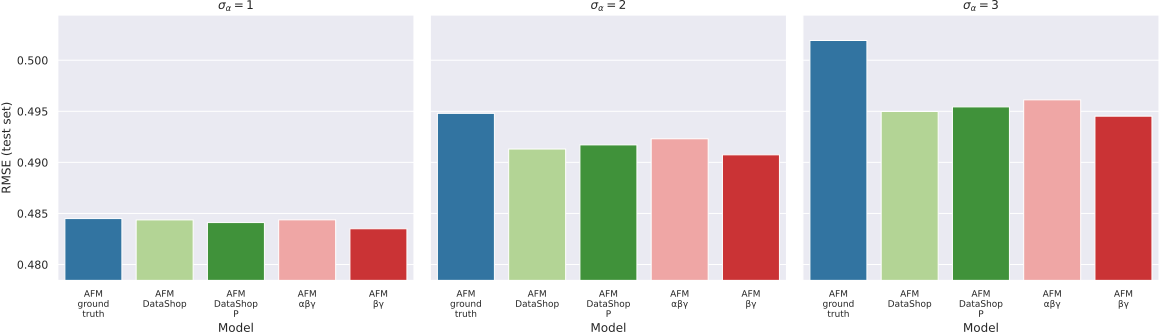
\includegraphics[width=0.72\linewidth]{figures/rmse_test}
		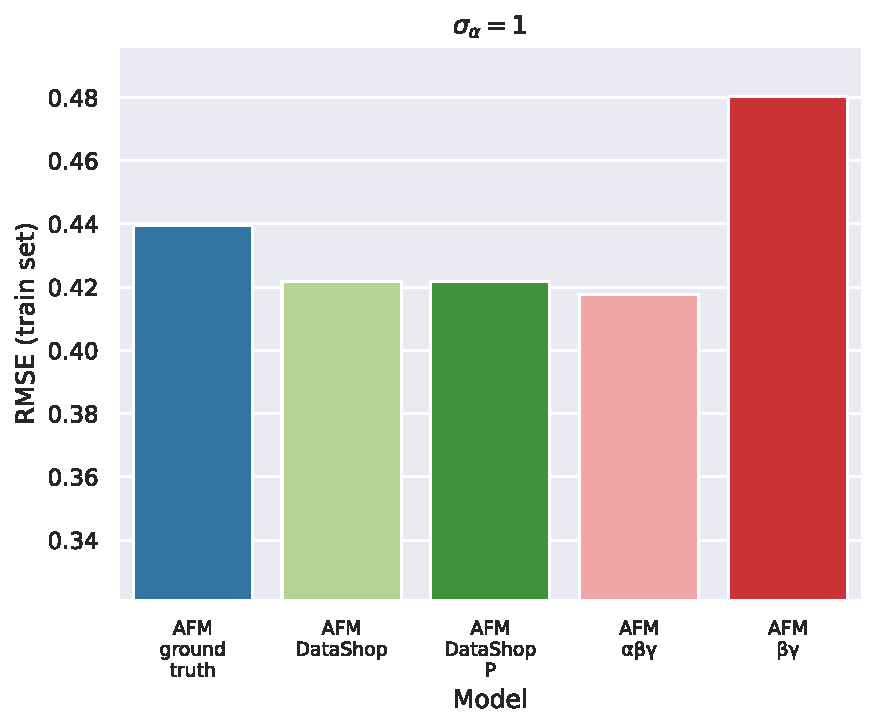
\includegraphics[width=0.25\linewidth]{figures/alpha_1_beta_neg0.5_complete_random_rmse_train}
	\end{center}
\end{frame}

\begin{frame}
	\frametitle{Results}
	Fitted parameters diverge from the ground truth parameters (closer to zero).
	
	\begin{center}
		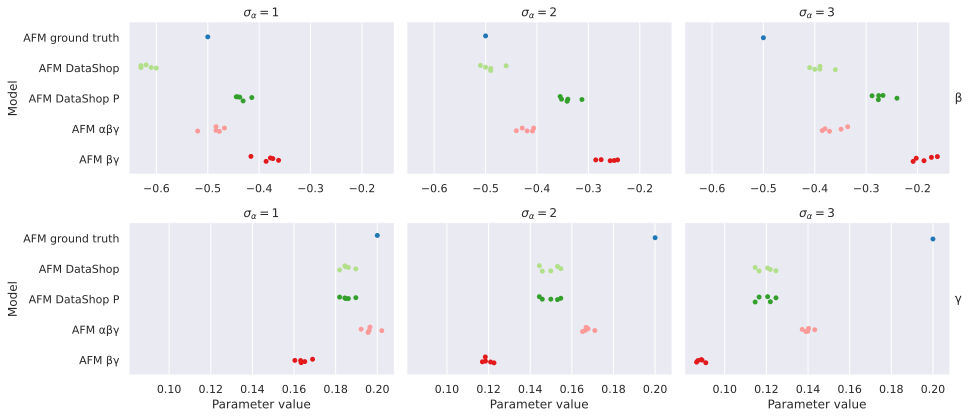
\includegraphics[width=0.99\linewidth]{figures/afm_params_comparison_both}
	\end{center}
\end{frame}


\begin{frame}
	\frametitle{Explanation}
	Logistic function skews the distribution when transforming logits to probabilities.\\
	Skewed probability distribution has expected value closer to zero.\\
	Distributions with lower variance (narrower) are less skewed.
	\begin{center}
		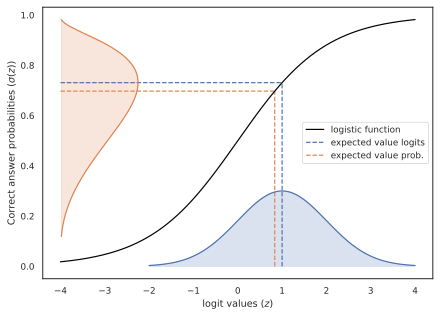
\includegraphics[width=0.48\linewidth]{figures/normal_sigma_skewed_n_1_1}
		\hspace*{.2em}
		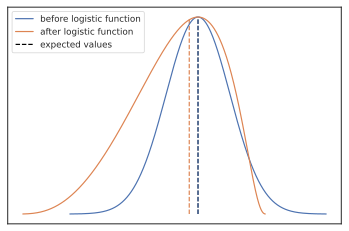
\includegraphics[width=0.475\linewidth, trim = 0cm -0.8cm 0cm 0cm]{figures/distribution_shift}
  	\end{center}
\end{frame}

\begin{frame}
	\frametitle{Explanation}	
	Best RMSE is achieved when predicting the point estimate of expected value of probability distribution 
	\\
	$\Rightarrow$ parameters closer to zero result in better point estimate of expected value.
	
	Fitted $\alpha$ parameters are regularized resulting in narrower estimate $\alpha$ distribution that is 
	less skewed by logistic function \\
	$\Rightarrow$ $\beta$ and $\gamma$ parameters shifted towards zero to maximize likelihood.
\end{frame}

\begin{frame}
\frametitle{Message}
\begin{enumerate}
\item Fitted models have to be interpreted carefully.
\bigskip
\item Implementation details matter. 
\end{enumerate}
\end{frame}

\begin{frame}[standout]
	\frametitle{}
	\begin{center}
		Thank you for your attention.
	\end{center}
	\vfill
	{
		\raggedright
		\footnotesize
		Better Model, Worse Predictions: The Dangers in Student Model Comparisons\\
		J. Čechák, R. Pelánek
		
	}

\end{frame}


\end{document}
